\chapter{Performance evaluation of cached}\label{ch:cached-evaluation}

\begin{flushright}
	\textit{"There are three kinds of lies:\\
		lies, damned lies, \\
		and \sout{statistics} benchmarks."}	\\

	Mark Twain (modernized)
\end{flushright}

It may seem as an ironic statement, considering that we are about to provide 
benchmark results for cached, but it's actually is a valid one. What Mr.  Twain 
tries to say here
\footnote{
	and that's a phrase usually not heard in programming contexts...
}
is that the presentation of partials facts for something can be used to 
fabricate a plausible truth for it.
%This is shit, fix it
In science's case, it so often happens that promising results for an experiment 
can seem more important to the researcher's eye than negative ones due to 
positive reinforcement.

In out case, we will try not to merely smear the next pages with diagrams but 
first explain the benchmarking methodology behind them.

The skeleton of this chapter is the following: Section \ref{sec:perf-meth} 
explains the methodology behind our measurements. Section \ref{sec:perf-plot} 
presents the results of the benchmarks that we have done and provides in-depth 
explanations about each of them. Finally, Section ? is undefined.

\section{Benchmark methodology}\label{sec:perf-meth}

The benchmarks that have been executed and whose results are presented in this 
chapter, will be split in two categories, both of which have their own distinct 
goals:

The first category is the comparison between using cached on top of the sosd 
(sosd has been discussed here ?) and using solely the sosd as the Archipelago 
storage. The category's goal is to "defend" one of the core thesis arguments, 
that tiering is a key element that will improve the performance of Archipelago. 

In order to compare effectively the performance of cached and sosd, we must 
consider the following: 

\begin{enumerate}
	\item The comparison of the two peers should try to focus on what is 
		the best performance that these peers can achieve for a series 
		of tough workloads.
	\item The circumstances under which both peers will be tested need not 
		be thorough but challenging. For example, it may be interesting 
		to test both peers against sequential requests, but
		\begin{inparaenum}[i)]
		\item such patterns are rarely a nuisance for production 
			environments
		\item they do not stress the peers enough to provide something 
			conclusive
		\item they are out of the scope of this section as there can be 
			many of them and adding them all here will impede the 
			document's readability.
		\end{inparaenum}
		
	\item Both peers must be tested under the same, reasonable workload, 
		i.e a workload that can be encountered in production 
		environments.
	\item If the peer doesn't show a consistent behavior for a workload, it 
		must be depicted in the results.
\end{enumerate}

Having the above in mind, the next step is to choose a suitable workload.  This 
choice though is fairly straight-forward; in production environments, the most 
troublesome workload is the stampede of small random reads/writes and is 
usually the most tested scenario.  

One may ponder however, how many requests can be considered as a "stampede" or 
which block size is considered as "small". Of course, there is not only one 
answer to this question so, we will work with ranges. For our workload, we will 
use block sizes ranging from 4KB to 64KB and parallel requests ranging from 4 
to 16.

The second category deals solely with the inner-workings of cached and its 
behavior on different operation modes or states. Its aim is not to capture the 
performance against a tough workload, but to explain \textbf{why} this 
performance is observed and how each of the options affect it. For example, we 
will measure things (blarg?) such as writethrough mode vs writeback mode, 
single-threaded vs multi-threaded etc.

Also, here is the following list is the options of cached that affect the 
measurements: 

\begin{enumerate}
	\item Bucket size
	\item IOdepth
	\item Cache size
	\item Max cached objects
	\item Write policy
	\item ...
\end{enumerate}

Finally, in the following sections for brevity reasons we will talk about 
comparing cached and sosd. What the reader must keep in mind however is that 
cached is the cache layer above sosd. 

\section{Performance comparison between cached and sosd}

As mentioned above, for our first test, we will evaluate the read and write 
performance of cached and sosd (in bandwidth and latency) for a random workload 
with parallel requests of small size. The results can be seen in Figure 
\ref{fig:comp-lie}. 

\begin{figure}[hb]
	\centering
	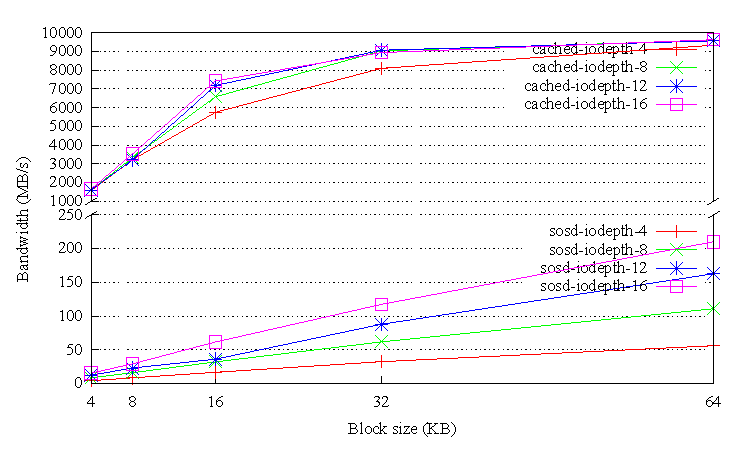
\includegraphics[]{diagrams/bw-write-comp-lie.pdf}
	\caption{Bandwidth performance for write}
	\label{fig:bw-write-comp-lie}
\end{figure}

\begin{figure}[hb]
	\centering
	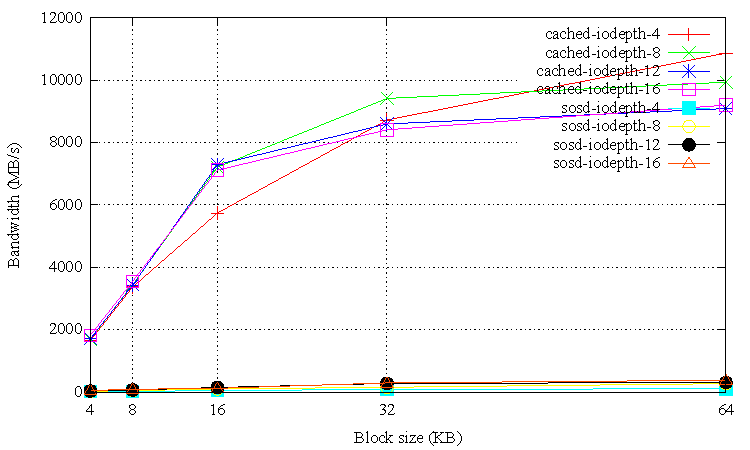
\includegraphics[]{diagrams/bw-read-comp-lie.pdf}
	\caption{Bandwidth performance for read}
	\label{fig:bw-read-comp-lie}
\end{figure}

